%&../../.preamble
\endofdump

\lstdefinelanguage{lua}{
  classoffset = 1, keywordstyle = \textbf,
  morekeywords={
and, break, do, else, elseif, end, false, for, function, if, in, local, nil, not, or, repeat, return, then, true, until, while
  },
    %
  classoffset = 2, keywordstyle = \textit,
  classoffset = 0,
  morecomment=[l]{--},
  morecomment=[s]{--[[}{]]--},
  morestring=[b]",
  morestring=[d]',
  stringstyle = \color{string},
  commentstyle = \color{comment}\textit
}

\geometry{margin=20mm}
\usetikzlibrary{external}
\tikzset{external/system call={pdflatex --shell-escape --fmt=../.preamble --halt-on-error -jobname "\image" "\endofdump\texsource"}}
\tikzexternalize[prefix=tikz/]

\begin{document}
\begin{minipage}[t]{0.48\textwidth}
	\subsubsection*{Graphs}
	\begin{itemize}
		\item {\ttfamily G.n} %- numero di nodi
		\item {\ttfamily G.adj(x)}% - ritorna i vicini di \verb|x|
		\item {\ttfamily distance(G, x, v)} - lancia bfs a partire da \verb|x| e salva i risultati in \verb|v|
		\item {\ttfamily NODE n} %- dichiara un nodo di \verb|g|. Corrisponde ad un intero
    \item \verb| G.insertNode(u)|% inserisce il nodo \verb|u| in \verb|g|
    \item \verb| G.insertEdge(u, v)|% inserisce un arco fra \verb|u| e \verb|v|
	\end{itemize}
  \vskip3mm
  \subsubsection*{Stack}
  \begin{itemize}
    \item \verb|STACK s = new STACK()|% inizializzzazione
    \item \verb|s.push(x)| %inserisce \verb|x| nello stack
    \item \verb|s.pop()| %rimuove l'ultimo elemento e lo ritorna come valore
    \item \verb|s.top()| %ritorna l'utlimo elemento ome valore
    \item \verb|s.isEmpty()| %ritorna \verb|true| se lo stack è vuoto
  \end{itemize}
  \subsubsection*{Tree}
  \begin{itemize}
    \item \verb|TREE T = new TREE()|
    \item \verb|T.left()|
    \item \verb|T.right()|
    \item \verb|count(TREE T)| ritorna il numero di nodi dell'albero
    \item \verb|T.deleteLeft()|
    \item \verb|T.deleteRight()|
  \end{itemize}
\end{minipage}
%
\begin{minipage}[t]{0.48\textwidth}
  \subsubsection*{Queue}
  \begin{itemize}
    \item \verb|QUEUE q = new QUEUE()| %- inizializzazione
    \item \verb|q.enqueue(x)| %- aggiunge \verb|x|
    \item \verb|q.dequeue()| %- rimuove l'ultimo elemento e lo ritorna come valore
    \item \verb|q.top()| %- ritorna l'elemento in testa alla coda
  \end{itemize}
  \vskip3mm
  \subsubsection*{Set} 
 \begin{itemize}
    \item \verb|SET s = new SET()|
    \item \verb|s.size()|
    \item \verb|s.contains(ITEM i)|
    \item \verb|s.insert(ITEM i)|
    \item \verb|s.remove(ITEM i)|
    \item \verb|union(SET a, SET b)|
    \item \verb|intersection(SET a, SET b)|
    \item \verb|difference(SET a, SET b)|
 \end{itemize}

  \subsubsection*{Dictionary}
  \begin{itemize}
    \item \verb|DICTIONARY d = new DICTIONARY()|
    \item \verb|d.lookup(ITEM i)|
    \item \verb|d.insert(ITEM key, value)|
    \item \verb|d.remove(ITEM key)|
  \end{itemize}

\end{minipage}
\newpage  


\begin{minipage}[c]{0.58\textwidth}
\begin{lstlisting}[language = lua, frame = none, numbers = none]
local function lowerBound(v, k, i, j)
    if i == j then return i end

    local m = math.floor((i+j)/2)

    if v[m] >= k then
      return lowerBound(v, k, i, m)
    else
      return lowerBound(v, k, m+1, j)
    end
end
\end{lstlisting}
\end{minipage}
%
\begin{minipage}[c]{0.38\textwidth}
  \underline{Ritorna il primo indice in cui si trova l'elemento k}
  \vskip3mm 
  Se \verb|k| non è presente nel vettore, allora viene ritornato l'indice in cui andrebbe inserito per mantenere l'ordinamento. \underline{NON considera casi in cui l'elemento va inserito all'inizio o alla fine}
\end{minipage}
\vskip3mm
\hrule
\begin{minipage}[c]{0.58\textwidth}
  
\begin{lstlisting}[language = lua, frame = none, numbers = none]
local function upperBound(v, k, i, j)
  if i == j then return i end

  local m = math.ceil((i+j)/2)

  if v[m] > k then
    return upperBound(v, k, i, m-1)
  else
    return upperBound(v, k, m, j)
  end
end
\end{lstlisting}
\end{minipage}
%
\begin{minipage}[c]{0.38\textwidth}
  \underline{Ritorna l'ultimo indice in cui si trova l'elemento k}
\end{minipage}

\vskip3mm
\hrule
\begin{center}
  \begin{lstlisting}[language = lua, frame = none, numbers = none]
  local function bfs(graph, start)
  local queue = {}
  local distances = {}

  for i = 1, graph.size do
    distances[i] = -1
  end

  distances[start] = 0
  table.insert(queue, start)

  while #queue ~= 0 do
    local currVertex = queue[1]
    table.remove(queue, 1)
    for _, vTo in ipairs(graph[currVertex]) do
      if distances[vTo] == -1 then
        distances[vTo] = distances[currVertex] + 1
        table.insert(queue, vTo)
      end
    end
  end
  return distances
end
\end{lstlisting} 
\end{center}
\hrule
\begin{center}
\begin{lstlisting}[language = lua, frame = none, numbers = none]
local function locateRec(t, index, level, pos)

  if t == nil then return nil end

  if t.index==index then return level, pos end

  local levelL, posL = locateRec(t.left, index, level+1, 2*pos)
  if levelL then return levelL, posL end

  local levelR, posR = locateRec(t.right, index, level+1, 2*pos +1)
  if levelR then return levelR, posR end

  return nil

end
  \end{lstlisting} 
\end{center}
\begin{center}
  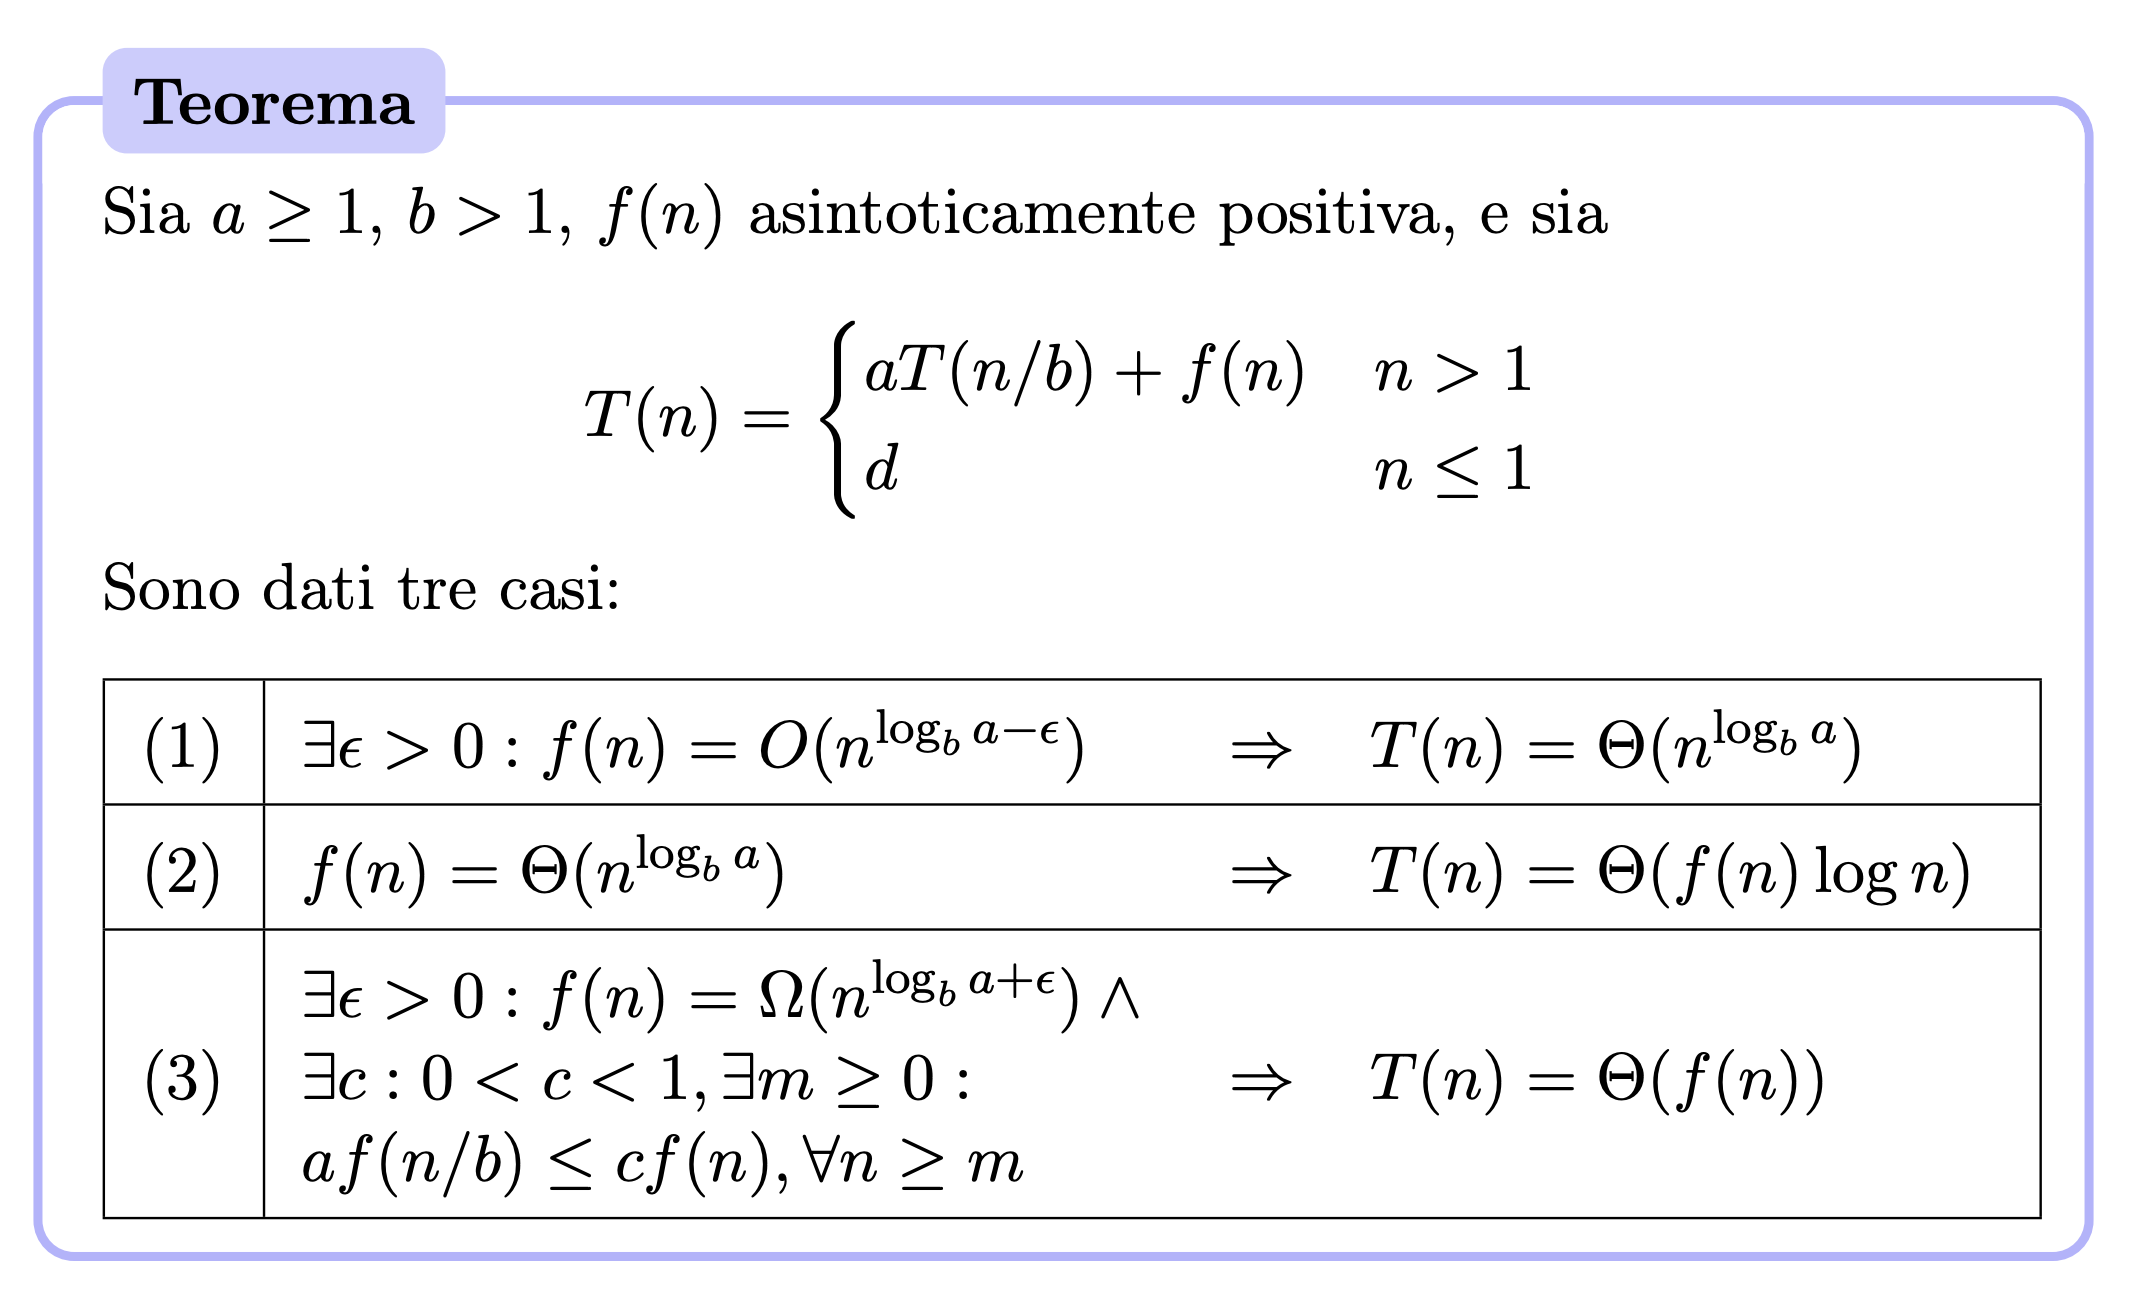
\includegraphics[width=\textwidth]{images/MASTER.png }
\end{center}


\end{document}
